\documentclass[9pt]{beamer}
\usetheme{Luebeck}
%\usecolortheme{seahorse}
\useinnertheme{rectangles}
\useoutertheme{infolines}
\usepackage{xcolor}
\usepackage[utf8]{inputenc}
\usepackage{tikz}
\usepackage{tabularx}
\usepackage[]{color}
\usepackage{lipsum}
\usepackage{amsmath,graphicx,dsfont}
\usetikzlibrary{shapes,backgrounds,arrows,automata,snakes,shadows,positioning, mindmap}
%===================================
\newcommand{\backupbegin}{
   \newcounter{framenumberappendix}
   \setcounter{framenumberappendix}{\value{framenumber}}
}
\newcommand{\backupend}{
   \addtocounter{framenumberappendix}{-\value{framenumber}}
   \addtocounter{framenumber}{\value{framenumberappendix}} 
}

\makeatletter
\setbeamertemplate{footline}
{
  \leavevmode%
  \hbox{%
  \begin{beamercolorbox}[wd=.333333\paperwidth,ht=2.25ex,dp=1ex,center]{author in head/foot}%
    \usebeamerfont{author in head/foot}\insertshortauthor%~~\beamer@ifempty{\insertshortinstitute}{}{(\insertshortinstitute)}
  \end{beamercolorbox}%
  \begin{beamercolorbox}[wd=.333333\paperwidth,ht=2.25ex,dp=1ex,center]{title in head/foot}%
    \usebeamerfont{title in head/foot}\insertshorttitle
  \end{beamercolorbox}%
  \begin{beamercolorbox}[wd=.333333\paperwidth,ht=2.25ex,dp=1ex,right]{date in head/foot}%
    \usebeamerfont{date in head/foot}\insertshortdate{}\hspace*{2em}
    \insertframenumber{} / \inserttotalframenumber\hspace*{2ex} 
  \end{beamercolorbox}}%
  \vskip0pt%
}
\makeatother
%===================================
\definecolor{Framableu}{RGB}{12,91,122}
\definecolor{Framableulight}{RGB}{18,144,176}
\definecolor{Nicered}{RGB}{176,18,65}
%\definecolor{Nicered}{RGB}{141,14,52}
\definecolor{Lightpink}{RGB}{229,177,218}
\definecolor{Green}{RGB}{144,176,18}
\definecolor{Lightcomplement}{RGB}{235,204,196}
\definecolor{Darkgoldenrod}{RGB}{176,144,18}
\definecolor{Darkomplement}{RGB}{122,43,12}
\definecolor{Complement}{RGB}{176,50,18}
\definecolor{Darkgreen}{RGB}{52,141,14}
\definecolor{Framavert}{RGB}{0, 182, 124} % Framavert
\definecolor{green2}{RGB}{121, 155, 0}
%===================================
\setbeamertemplate{itemize items}[square]
\setbeamertemplate{blocks}[shadow=false]
\setbeamertemplate{caption}{\raggedright\insertcaption\par}
%===================================
\setbeamercolor{section in head/foot}{fg=white,bg=Framableu}
\setbeamercolor{subsection in head/foot}{fg=white,bg=Framableulight}
\setbeamercolor{author in head/foot}{bg=Framableu}
\setbeamercolor{item}{fg=Framableulight}
\setbeamercolor*{structure}{bg=Framableulight!20,fg=Framableulight}
\setbeamercolor*{palette secondary}{use=structure,fg=white,bg=structure.fg!75}
\setbeamercolor{section in toc}{fg=Framableu,bg=white}
\setbeamercolor{frametitle}{fg=Framableu!80,bg=white}
\setbeamercolor{block title}{fg=white, bg=Framableulight}  
\setbeamercolor{block title example}{fg=white, bg=green2}  
%===================================
\title{Mixture tree model for network inference}

\institute[]
{  \inst{1}%
  UMR AgroParisTech / INRA MIA-Paris \\
  \inst{2}%
  LaMME, Evry
  }
\date{July 10, 2018}
 
\author{Raphaëlle Momal} 
\newcommand{\Ccal}{\mathcal{C}}
\newcommand{\edgeunit}{1.5}
\newcommand{\emphase}[1]{\textcolor{Complement}{#1}}
\newcommand{\bleu}[1]{\textcolor{Framableulight}{#1}}
\newcommand{\pos}[1]{\textcolor{Darkgreen}{#1}}
\newcommand{\nega}[1]{\textcolor{Nicered}{#1}}
\newcommand\independent{\protect\mathpalette{\protect\independenT}{\perp}}\def\independenT#1#2{\mathrel{\rlap{$#1#2$}\mkern2mu{#1#2}}}
\newcommand{\Ncal}{\mathcal{N}}
\tikzset{%
    observed/.style={%
    scale=0.6,circle,draw=Framableulight,transform shape,fill=white,font=\Large}
}
\newcommand{\argmax}{\mathop{\mathrm{argmax}}}   
%#################################################################
\begin{document}
%\AtBeginSection[]{
%   \begin{frame}
   %%% affiche en début de chaque section, les noms de sections et
   %%% noms de sous-sections de la section en cours.
%   \tableofcontents[currentsection,hideothersubsections]
%   \end{frame} 
%}
\begin{frame}
    \titlepage
\begin{center}
\vspace{-1cm}
	
\includegraphics[width=0.25\linewidth]{logo_inra.jpg}\hspace{0.1cm}
	
\includegraphics[width=0.25\linewidth]{agro.PNG}
	
\includegraphics[width=0.25\linewidth]{lmh.png}\hspace{0.1cm}
	
\includegraphics[width=0.15\linewidth]{upsud.jpg}
    
\end{center}
\end{frame}

\begin{frame}{CV}
\begin{tabular}{c l}

\includegraphics[scale=0.07]{logo_inra}&  Final internship, multi-OMICS data analysis (Jouy)\\
& avril 2017 - octobre 2017 \\
     
\includegraphics[scale=0.25]{logo_univ.jpg}& Mathematical statistics Research MSc (Rennes) \\
     &2016-2017 \\
    
\includegraphics[scale=0.4]{logo_ensai.jpg} & Preparation of biostatician ingeneer diploma (Rennes)\\
    & 2014-2017\\
    
\includegraphics[scale=0.25]{Logo-SL.png} & Prep school MPSI/MP, St Louis highschool (Paris)
\\
&2012-2014\\
\end{tabular}
\end{frame}
\section{Motivation}
%====================================================================
%====================================================================
\section{Thesis related activities}
\begin{frame}{Training courses}
    \begin{description}
    \item[Cross training]53h\begin{itemize}
    
        \item Basis for teaching
        \item Journées Carrières en Mathématiques
        \item Career plan definition (FEM and course)
        \item[]
    \end{itemize}
    \item[Pedagogical] M2 "Mathématiques pour les Sciences du vivant", Orsay\begin{itemize}
        
        \item Statistiques en grande dimension - C.Giraud
        \item Models with Hidden Structure - S. RObin
    \end{itemize}
    \end{description}
\end{frame}
%====================================================================
%====================================================================
\begin{frame}{Doctoral mission}
    50\% teaching - 50\% scientific mediation:\\\vspace{1cm}
    
    \begin{description}
    \item[Teaching] Statistical data interpretation with R (26h, L3 MINT Orsay)\bigskip
    \item[Mediation] MISS - Maison d'Initiation et de Sensibilisation aux Sciences (12 days per year, 8-15 years-old)
    \begin{itemize}
    \item Mathématiques et botanique
    \item Histoire des nombres
    \end{itemize}
    
    \end{description}
\end{frame}
%====================================================================
%====================================================================

\begin{frame}{Talks}
    This work was presented in : \vspace{0.5cm}
\begin{description}
    \item[Research schools:] \begin{itemize}
        \item []
        \item Scientific seminar, Rochebrune, 25-30 March
        \item Chaire MMB (Modélisation Mathématique et Biodiversité), Aussois, 12-16 May\bigskip
    \end{itemize}
    \item[Conference:] JOBIM (Journées Ouvertes de Biologie Informatique \& Mathématiques), 3-6 July
\end{description}
\end{frame}
%====================================================================
%====================================================================

\section{}
\subsection{}
\begin{frame}{}
\begin{center}
\huge{\bleu{The subject: preliminaries and general approach}}
\end{center}
\end{frame}
\section{Motivation}


\begin{frame}{Context}

Rising interest in \emphase{jointly analysed }species abundances:
\begin{itemize}
	\item Metagenomics 
	\item Microbiology
	\item Ecology
\end{itemize}
%\pause

\begin{block}{Ecological network}
Tool to better understand species interactions (direct/indirect), eco-systems organizations (clusters ?) 
\end{block}\bigskip
%\pause
Allows for resilience analyses, pathogens control, ecosystem comparison, response prediction...
\end{frame}
%====================================================================
%====================================================================


\begin{frame}{Data example}
	\begin{itemize}
	\item \emphase{Species}: bacteria, fungi...
	\item \emphase{Abundances}: read counts from Next-Generation Sequencing technologies (metabarcoding)
	\item \emphase{Covariates}: sequencing depth, temperature, water depth...  \bigskip
	
\end{itemize}
	Repeated signal : $n$ samples, $p$ abundances.
%\pause
\begin{block}{Data table}
	$Y = [Y_{ij}]_{(i,j) \in \{1,...,n\} \times \{1,..., p\}} $
	\begin{itemize}
	\item $Y_{ij}$: abundance of the $j^{th}$ species in the $i^{th}$ sample
\end{itemize}
\end{block}
\begin{center}
	Infer the \emphase{species interaction network} from count data $Y$
\end{center}
\end{frame}
%====================================================================
%====================================================================
\begin{frame}{Challenges}\large{
	\begin{itemize}
	\item  Statistical network inference \bigskip\bigskip
	\item Count data \bigskip\bigskip
	\item Offsets and covariates
\end{itemize}}
\end{frame}
%====================================================================
%====================================================================

\section{Network inference}
\subsection{General Framework}
%====================================================================
%===================================================================

\begin{frame}{Graphical models: a statistical framework for network inference}
\bleu{Example}:\bigskip
\begin{columns}
\begin{column}{0.3\linewidth}\hspace{0.5cm}
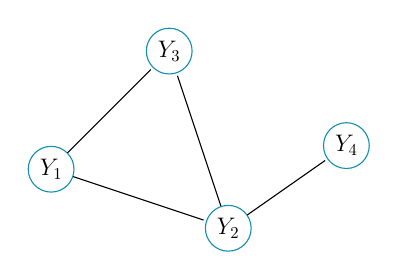
\begin{tikzpicture}	

      \tikzstyle{every edge}=[-,>=stealth',shorten >=1pt,auto,thin,draw]
		\node[observed] (Y1) at (0*\edgeunit, 0*\edgeunit) {$Y_1$};
		\node[observed] (Y2) at (1.5*\edgeunit, -0.5*\edgeunit) {$Y_2$};
		\node[observed] (Y3) at (1*\edgeunit, 1*\edgeunit) {$Y_3$};
		\node[observed] (Y4) at (2.5*\edgeunit, 0.2*\edgeunit) {$Y_4$};
		\path (Y1) edge [] (Y2)
        (Y1) edge [] (Y3)
        (Y2) edge [] (Y3)
        (Y2) edge [] (Y4);
	\end{tikzpicture}\\
\end{column}
\begin{column}{0.5\linewidth}
	\begin{itemize}
	\item All variables are dependant \bigskip
	\item Some are \emphase{conditionally independent} (i.e. indirectly dependeant)\\\bigskip
	 $Y_4$ is independent from $(Y_1, Y_3)$ conditionally on $Y_2$
\end{itemize}
\end{column}
\end{columns}

\end{frame}
%====================================================================
%====================================================================

\begin{frame}{Graphical models}
\begin{block}{Definition \cite{Lau96}}
	The joint distribution P is faithful to the graph G iff \[ P(Y_1, \dots, Y_p) \propto \prod_{C \in \Ccal_G} \psi_C(Y_C) \]
  where $\Ccal_G =$ set of maximal cliques of $G$.
\end{block}
%\pause
\begin{columns}
\begin{column}{0.4\linewidth}
\flushright
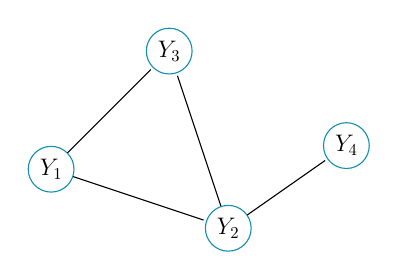
\begin{tikzpicture}	

      \tikzstyle{every edge}=[-,>=stealth',shorten >=1pt,auto,thin,draw]
		\node[observed] (Y1) at (0*\edgeunit, 0*\edgeunit) {$Y_1$};
		\node[observed] (Y2) at (1.5*\edgeunit, -0.5*\edgeunit) {$Y_2$};
		\node[observed] (Y3) at (1*\edgeunit, 1*\edgeunit) {$Y_3$};
		\node[observed] (Y4) at (2.5*\edgeunit, 0.2*\edgeunit) {$Y_4$};
		\path (Y1) edge [] (Y2)
        (Y1) edge [] (Y3)
        (Y2) edge [] (Y3)
        (Y2) edge [] (Y4);
	\end{tikzpicture}\\
\end{column}
\begin{column}{0.6\linewidth}
\begin{align*}
	P(Y_1, &Y_2, Y_3, Y_4) \propto \\ 
	& \psi_1(Y_1 ,Y_2, Y_3) \times \psi_2(Y_3, Y_4)
\end{align*} 
\end{column}
\end{columns}
\end{frame}

\subsection{Using trees}
%====================================================================
%====================================================================

\begin{frame}{Spanning trees}
	Unconstrained graph $\Rightarrow$ very large space to explore: \emphase{$\text{\#} \mathcal{G}_p = 2^{\frac{p(p-1)}{2}}$}\\ \bigskip
	
	Spanning trees are a \bleu{sparse} solution :
	$$
  \left. \begin{tabular}{l}
          $G$ is connected \\
          $G$ has no cycle
         \end{tabular} \right\}
  \text{ $G$ has $(p-1)$ edges}
  $$
  \begin{columns}
  \begin{column}{6cm}
	\begin{figure}[htp]
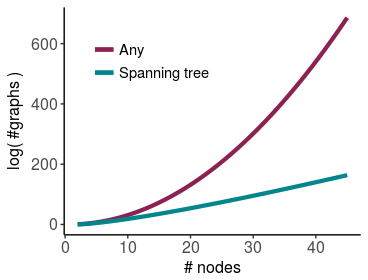
\includegraphics[width=5cm]{compar_typegraphs.png}
	\end{figure}
	\end{column}
	 \begin{column}{6cm}
Much \bleu{ smaller space} to explore:\\  \emphase{$$\text{\#} \mathcal{T}_p = p^{(p-2)}$$}\\ \bigskip
\pause
Still a huge complexity...
\end{column}
\end{columns}
\end{frame}


%====================================================================
%====================================================================
\begin{frame}{Maximizing and summing over spanning trees}
\begin{description}
\item[Maximum spanning tree] Kruskal's algorithm\\
 $$ \hat{T} = \emphase{\underset{T}{\mathrm{argmax }}}\left\{\prod_{(k,l) \in T} \psi_{k,l}(Y) \right\}  \rightarrow \emphase{\Theta (p^2 \log(p))}$$ \bigskip 
\item[Tree averaging] Matrix tree theorem \cite{matrixtree}\\ 
$$\emphase{ \sum_T}\prod_{(k,l) \in T} \psi_{k,l}(Y) = \det(L(Y))  \rightarrow \emphase{\Theta (p^3)}$$
\end{description}\pause \bigskip 
\center{
\textbf{Approach}: infer the network by \emphase{averaging spanning trees}}
	
\end{frame}


\begin{frame}{Tree structured data}
\begin{columns}
 \begin{column}{0.7\linewidth}
 \begin{itemize}
    \item Data dependency structure relies on a tree \vspace{1cm}
    \item Likelihood \emphase{factorizes on nodes and edges} \cite{ChowLiu}:
    \end{itemize}
 \end{column}
 \begin{column}{0.3\linewidth}
 \begin{center}
     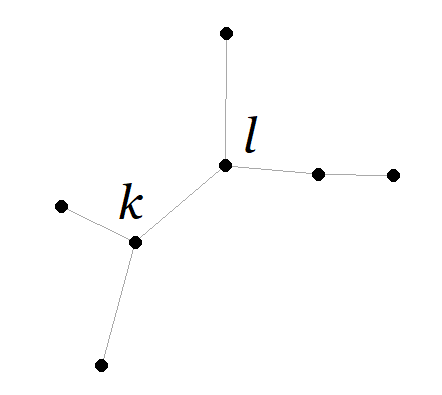
\includegraphics[width=3cm]{arbredependance.PNG}   
    \end{center}
 \end{column}
\end{columns}

\[\mathds{P}(Y|T) =\prod_{j=1}^d \mathds{P}(Y_j)\prod_{k,l \in T}\psi_{kl}(Y) \hspace{0.3cm},\]

Where \[ \psi_{kl}(Y) = \frac{\mathds{P}(Y_k,Y_l)}{\mathds{P}(Y_k)\times \mathds{P}(Y_l)}.\]\\
\vspace{0.4cm}
\textbf{Rmq} : with standardised gaussian data, $\hat{\Psi} = [\hat{\psi_{kl}}] \propto (1-\hat{\rho}^2)^{-1/2}$
\end{frame}

%====================================================================
%====================================================================

\begin{frame}{Tree averaging} 
\begin{center}
    

%\begin{tabular}{p{\linewidth}}
%\begin{tabularx}{\linewidth}{ccccl}
 \begin{tabular}{ccccl}
   \begin{tabular}{c}
	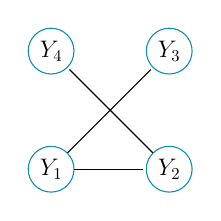
\begin{tikzpicture}
		
      \tikzstyle{every edge}=[-,>=stealth',shorten >=1pt,auto,thin,draw]
    
		\node[observed] (Y1) at (0*\edgeunit, 0*\edgeunit) {$Y_1$};
		\node[observed] (Y2) at (1*\edgeunit, 0*\edgeunit) {$Y_2$};
		\node[observed] (Y3) at (1*\edgeunit, 1*\edgeunit) {$Y_3$};
		\node[observed] (Y4) at (0*\edgeunit, 1*\edgeunit) {$Y_4$};
		\path (Y1) edge [] (Y2)
        (Y1) edge [] (Y3)
        (Y2) edge [] (Y4);
   
	\end{tikzpicture}\\
	\footnotesize{$P\{T = T_1 | Y\}$}
	   \end{tabular}
	   & 
	 %  \hspace{-.05\textwidth}% \pause
	   \begin{tabular}{c}
		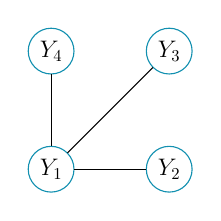
\begin{tikzpicture}
		\tikzstyle{every observed}=[draw=none,text=black,scale=0.5,
      transform shape,circular drop shadow] 
		\node[observed] (Y1) at (0*\edgeunit, 0*\edgeunit) {$Y_1$};
		\node[observed] (Y2) at (1*\edgeunit, 0*\edgeunit) {$Y_2$};
		\node[observed] (Y3) at (1*\edgeunit, 1*\edgeunit) {$Y_3$};
		\node[observed] (Y4) at (0*\edgeunit, 1*\edgeunit) {$Y_4$};
		
		\path (Y1) edge [] (Y2)
        (Y1) edge [] (Y3)
        (Y1) edge [] (Y4);
		\end{tikzpicture} \\
		\footnotesize{$P\{T = T_2 | Y\}$}
	   \end{tabular}
	   &
	  % \hspace{-.05\textwidth} %\pause
	   \begin{tabular}{c}
		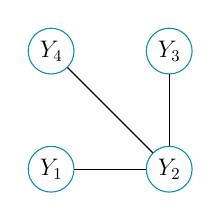
\begin{tikzpicture}
		\tikzstyle{every observed}=[draw=none,text=black,scale=0.5,
      transform shape,circular drop shadow] 
		\node[observed] (Y1) at (0*\edgeunit, 0*\edgeunit) {$Y_1$};
		\node[observed] (Y2) at (1*\edgeunit, 0*\edgeunit) {$Y_2$};
		\node[observed] (Y3) at (1*\edgeunit, 1*\edgeunit) {$Y_3$};
		\node[observed] (Y4) at (0*\edgeunit, 1*\edgeunit) {$Y_4$};
		
		\path (Y1) edge [] (Y2)
        (Y2) edge [] (Y3)
        (Y2) edge [] (Y4); 
		\end{tikzpicture}\\
		\footnotesize{$P\{T = T_3 | Y\}$}
	   \end{tabular}
	   &
	  % \hspace{-.05\textwidth}% \pause
	   \begin{tabular}{c}
		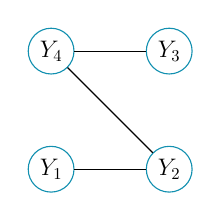
\begin{tikzpicture}
		\tikzstyle{every observed}=[draw=none,text=black,scale=0.5,
      transform shape,circular drop shadow] 
		\node[observed] (Y1) at (0*\edgeunit, 0*\edgeunit) {$Y_1$};
		\node[observed] (Y2) at (1*\edgeunit, 0*\edgeunit) {$Y_2$};
		\node[observed] (Y3) at (1*\edgeunit, 1*\edgeunit) {$Y_3$};
		\node[observed] (Y4) at (0*\edgeunit, 1*\edgeunit) {$Y_4$};
		 
		\path (Y1) edge [] (Y2)
        (Y3) edge [] (Y4)
        (Y2) edge [] (Y4);
		\end{tikzpicture} \\
		\footnotesize{$P\{T = T_4 | Y\}$}
	   \end{tabular}
	   & %\hspace{-.06\textwidth} 
	   \huge{\emphase{...}}\normalsize   \\ \\
	   \\% \pause
	   \begin{tabular}{l}
		Compute edge\\
		probabilities:
	   \end{tabular}
	   &
	  % \hspace{-.05\textwidth}
	   \begin{tabular}{c}
		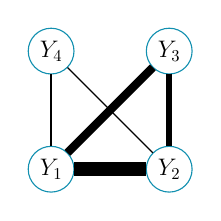
\begin{tikzpicture}
		\node[observed] (Y1) at (0*\edgeunit, 0*\edgeunit) {$Y_1$};
		\node[observed] (Y2) at (1*\edgeunit, 0*\edgeunit) {$Y_2$};
		\node[observed] (Y3) at (1*\edgeunit, 1*\edgeunit) {$Y_3$};
		\node[observed] (Y4) at (0*\edgeunit, 1*\edgeunit) {$Y_4$};
		\draw [line width=5pt] (Y1) -- (Y2); 
		\draw [line width=3pt] (Y1) -- (Y3); 
		\draw [line width=.5pt] (Y1) -- (Y4); 
		\draw [line width=2pt] (Y2) -- (Y3); 
		\draw [line width=.5pt] (Y2) -- (Y4); 
 %		\draw [line width=.5pt] (Y3) -- (Y4); 
		\end{tikzpicture}\\
		\emphase{$P\{(j, k) \in T | Y\}$}
	   \end{tabular}
	   &
	  % \hspace{-.05\textwidth} %\pause
	   \begin{tabular}{l}
		Thresholding\\
		probabilities:
	   \end{tabular}
	   &
	   %\hspace{-.05\textwidth}
	   \begin{tabular}{c}
		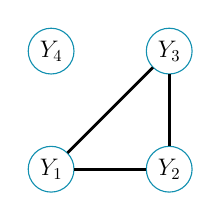
\begin{tikzpicture}
		\node[observed] (Y1) at (0*\edgeunit, 0*\edgeunit) {$Y_1$};
		\node[observed] (Y2) at (1*\edgeunit, 0*\edgeunit) {$Y_2$};
		\node[observed] (Y3) at (1*\edgeunit, 1*\edgeunit) {$Y_3$};
		\node[observed] (Y4) at (0*\edgeunit, 1*\edgeunit) {$Y_4$};
		\draw [line width=1pt] (Y1) -- (Y2); 
		\draw [line width=1pt] (Y1) -- (Y3); 
% 		\draw [line width=1pt] (Y1) -- (Y4); 
		\draw [line width=1pt] (Y2) -- (Y3); 
% 		\draw [line width=.1pt] (Y2) -- (Y4); 
% 		\draw [line width=1pt] (Y3) -- (Y4); 
		\end{tikzpicture}\\
		\emphase{$P\{(j, k) \in T | Y\}$}
	   \end{tabular}
	   &
	 \end{tabular}
   % \end{tabular}
   %\end{tabularx}
   \end{center}
\end{frame}
%====================================================================
%====================================================================


\section{With count data}
\subsection{Model}

%====================================================================
%====================================================================

\begin{frame}{PLN model}
\begin{block}{Poisson log-Normal distribution \cite{AiH89}}
\[
            \left.
                \begin{array}{rl}
               \vspace{0.2cm}    Z_i \textit{ iid } &\sim \mathcal{N}_{d}(0,\Sigma)\\
              \vspace{0.2cm}    &(Y_{ij})_j \independent |Z_i\\
                    Y_{ij}|Z_{ij} &\sim \mathcal{P}(e^{\only<2>{\emphase{o_{ij}+x_i^{\text{T}}\Theta_j} +}Z_{ij}}) 
                   
                \end{array}
            \right \} Y \sim \mathcal{PLN}(\only<2>{\emphase{O+X^{\text{T}}\Theta }}\only<1>{0}, \Sigma)  
            \]
\end{block}

\begin{itemize}
    \item Dependency structure in the Gaussian latent layer
    \item Easy handling of multi-variate data (contrary to Negative binomial distribution)
  \only<2>{ \item Allow adjustment for covariates and offsets}
  \only<2>{\item Variational estimation algorithm \cite{CMR17}}
\end{itemize}
%\pause

\end{frame}
%====================================================================
%====================================================================

\begin{frame}{PLN + mixture tree}
  %  \center{ \textbf{ Approach:} tree averaging to infer the \emphase{latent Gaussian network} }\
    $G$ is taken as a spanning tree $T$, the dependency structure is encoded in $\Sigma_T$.
    \[Z_T \sim \mathcal{N}(0,\Sigma_T) \]
    \\ \bigskip
    Tree averaging (mixture model):
    \[Z \sim \sum_T w_T \mathcal{N}(0,\Sigma_T)\]
    $$\Rightarrow \mathds{P}(Z) \propto \sum_T \prod_{k,l \in T} \beta_{k,l} \psi_{k,l}(Z_T)$$ 
\end{frame}
\section{}
\subsection{}
\begin{frame}{}
\begin{center}
\huge{\bleu{Detailed method}}
\end{center}
\end{frame}
%====================================================================
%====================================================================
\section{Statistical inference model}
\begin{frame}{Hierarchical model with latent tree }

\begin{enumerate}
    \item A spanning tree is drawn in a distribution decomposable on the edges:
   \begin{block}{Decomposable distribution for a tree $T$ \cite{MeilaJaak}}\normalsize{
    \[ \mathds{P}(T) = \frac{1}{B}\prod_{(k,l)\in T} \beta_{kl} \text{ , avec } B = \sum_{T\in\mathcal{T}} \prod_{(k,l)\in T} \beta_{kl} \]}
    \end{block}
\begin{itemize}
    \item A weight $\beta_{kl}$ is assign to each edge $(k,l)$
    \item The dependence tree probability is proportional to its weights product 
    \item We consider \emphase{varying weights}
\end{itemize}
\pause{
    \item \vspace{0.3cm} Data is simulated conditionally on the drawn tree :
    \[Z|T \sim \mathcal{N}_d(0, \Sigma_Z)\]}
\end{enumerate}
\pause{
\begin{center}
\vspace{0.5cm}
   The data shaping tree is treated as a  \emphase{latent variable}.\\
    \[\mathds{P}(Z)=\sum_{T \in \mathcal{T}} \mathds{P}(T) \mathds{P}(Z|T)\text{ : \emphase{mixture tree}}\]
\end{center}
}
    
\end{frame}

%====================================================================
%====================================================================



\section{EM algorithm}
\subsection{E step}
%====================================================================
%====================================================================

\begin{frame}{E step}

\begin{itemize}
    \item Complete likelihood :

 \[ \mathds{P}(Y,Z,T) = \color{olive}\mathds{P}(T)\color{black}\times\color{blue}\mathds{P}(Z|T)\color{black}\times\color{orange}\mathds{P}(Y|Z)\]
 
\begin{align*}
 \log(\mathds{P}(Y,Z,T)) &= \sum_{k,l} \mathds{1}_{\{(k,l) \in T\}} (\color{olive}\log(\beta_{kl})\color{black} + \color{blue}\log(\psi_{kl}(Z)) \color{black})-\color{olive}\log(B)\color{black} \\
 &+\sum_k (\color{blue} \log(\mathds{P}(Z_k))\color{black} + \color{orange}\log(\mathds{P}(Y_k|Z_k))\color{black})
 \end{align*}
 
 \pause
 \item Conditional expectation :

\begin{align*}
    \mathds{E}_\theta[\log(\mathds{P}(Y,Z,T))|Y] =&\sum_{k,l\in V} \mathds{P}((k,l) \in T|Y) \log(\beta_{kl}) + \mathds{E}[\mathds{1}_{\{(k,l) \in T\}}\emphase{\log(\psi_{kl}(Z)|Y)}]\\
& +\sum_k \emphase{\mathds{E}[\log(\mathds{P}(Z_k)) | Y]} + \mathds{E}[\log(\mathds{P}(Y_k|Z_k)) | Y]-\log(B)
\end{align*} 
\end{itemize}
\end{frame}
%====================================================================
%====================================================================


\begin{frame}{Two steps solution}
   The {\fontfamily{qcr}\selectfont
PLNmodels} package approximates the distribution parameters. Using {\fontfamily{qcr}\selectfont
PLNmodels}:
    \vspace{0.3cm}
    \begin{enumerate}
        \item Estimate $\hat{\Sigma}_Z$ \vspace{0.2cm}
        \item Apply EM mixture tree to $Z \sim \mathcal{N}(0,\hat{\Sigma}_Z)$\\
    \end{enumerate}
\vspace{1.5cm}
Simplified conditional expectation writing:\\
\vspace{0.2cm}
\[\mathds{E}_\theta[\log(\mathds{P}(Z,T))|Z] =\sum_{k,l}  \emphase{\mathds{P}((k,l) \in T|Z)}(\log(\beta_{kl}) + \log(\psi_{kl}) )-\log(B) +\sum_k \log(\mathds{P}(Z_k))\]
\end{frame}
%====================================================================
%====================================================================

\begin{frame}{Conditional probability computation}
\begin{exampleblock}{Kirchhoff's theorem (matrix tree, \cite{AiH89})}
For all $W=(a_{kl})_{k,l}$ a symmetric matrix, the corresponding Laplacian $Q(W)$ is defined as follows:
 \[\mathcal{Q}_{uv}(W)=
 \begin{cases}
     -a_{uv} & 1\leq u<v \leq n\\
    \sum_{i=1}^n a_{vi} & 1\leq u=v \leq n.
\end{cases}
\]
Then for all $u$ et $v$:
    \[ |Q^*_{uv}(W)|=\sum_{T\in\mathcal{T}} \prod_{\{k,l\}\in E_T} a_{kl} \]
\end{exampleblock}
\begin{align*}
  \mathds{P}((k,l)\in T | Z)&=\sum_{T\in \mathcal{T} : (k,l)\in T}\mathds{P}( T | Z) = \frac{\sum_{(k,l)\in T} \mathds{P}(T)\mathds{P}(Z|T)}{\sum_{T} \mathds{P}(T)\mathds{P}(Z|T)}\\
 &=1- \frac{|Q^*_{uv}(B\Psi^{-kl})|}{|Q^*_{uv}(B\Psi)|}\\
 &= \tau_{kl}
 \end{align*}
 
\end{frame}



%====================================================================
%====================================================================

\subsection{M step}
\begin{frame}{M step}
\textbf{Goal} : optimization of weights $\beta_{kl}$.\\
\vspace{1cm}
\[\argmax_{\beta_{kl}} \left\{\sum_{k,l\in V} \tau_{kl}(\emphase{\log(\beta_{kl})} + \log(\psi_{kl}) ) -\emphase{\log(B)} +\sum_k \log(\mathds{P}(Z_k))\right\}\]

  \vspace{1cm}
  
 \[\text{With high combinatorial complexity of } B = \sum_{T\in\mathcal{T}} \prod_{k,l\in T} \beta_{kl}\]
 
 \begin{center}
     How to compute \Large{$\frac{\partial B}{\partial\beta_{kl}}$ }?
 \end{center}
\end{frame}
 %====================================================================
%====================================================================

 \begin{frame}{$\beta_{kl}$ update}
 \begin{exampleblock}{A result from Meil{\u{a}} \cite{MixtTrees}}
Inverting a minor of the laplacien $Q$, we define M : 
\[\begin{cases}
    M_{uv} = [\mathcal{Q}^{*-1}]_{uu} + [\mathcal{Q}^{*-1}]_{vv} -2[\mathcal{Q}^{*-1}]_{uv} & u,v < n\\
    M_{nv} =M_{vn} =[\mathcal{Q}^{*-1}]_{vv} & v<n\\
     M_{vv} =0.
   \end{cases}\]
On peut montrer que :
\[ \frac{\partial|Q^*_{uv}(W)|}{\partial \beta_{kl}} = M_{kl} \times |Q^*_{uv}(W)|\]
\end{exampleblock}
\[ \frac{\partial\mathds{E}_\theta[\log(\mathds{P}(Z,T))|Z]}{\partial\beta_{kl}} =\frac{1 }{\beta_{kl}} \tau_{kl} - \frac{1}{B}
\frac{\partial B}{\partial\beta_{kl}}
\]


\begin{block}{Update formula at iteration $h+1$}
   \large{\[\hat{\beta}_{kl}^{h+1} = \frac{\tau_{kl}^h}{M_{kl}^h}\]}
   \end{block}
 \end{frame}
%====================================================================
%====================================================================
\section{Simulation}


\subsection{}
%====================================================================
%====================================================================

\begin{frame}{Simulation design}

\begin{enumerate}
     \item Choose  \emphase{$G$} and define  \emphase{$\Omega$} accordingly\vspace{0.3cm} 
     \item Sample count data \emphase{$Y$} from $\mathcal{PLN}(0,\Omega^{-1})$ with possible covariates
     \item Infer the network with \emphase{PLN + mixture tree EM}  and \emphase{SpiecEasi} \vspace{0.3cm}
     \item Compare results with \emphase{AUC} (presence/absence of edges)
\end{enumerate}\bigskip\bigskip
\hspace{1cm}$\Rightarrow$ 40 replicates for each setting $(p, n, \text{edge probability})$
	
\end{frame}

\subsection{Competitor}
%====================================================================
%====================================================================

\begin{frame}{Gaussian Graphical Models (GGM) }
   \emphase{Gaussian distribution:}\\
 \begin{center}
	$  Y_i \sim \Ncal_p(\mu, \Omega^{-1}) $, $\mu =$ vector of means, $\Omega^{-1} =$ precision matrix.

 % \[L(Y,\Omega) \propto \frac{n}{2}\log(det(\Omega))-\frac{n}{2} Y^T\Omega Y\]
\end{center}
  
 
  
   \bigskip %\pause
  \emphase{A nice property:} 
\begin{align*}
p(Y) &\propto exp(-Y^T \Omega Y /2)\\
&\propto \prod_{j,k, \omega_{jk} \neq 0 } exp(-Y_j \omega_{jk} Y_k /2)  
\end{align*}
  \begin{columns}
  \begin{column}{0.15\textwidth}
	
\end{column}
  \begin{column}{0.4\textwidth}
   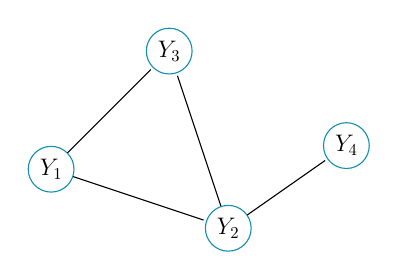
\begin{tikzpicture}	

       \tikzstyle{every edge}=[-,>=stealth',shorten >=1pt,auto,thin,draw]
		\node[observed] (Y1) at (0*\edgeunit, 0*\edgeunit) {$Y_1$};
		\node[observed] (Y2) at (1.5*\edgeunit, -0.5*\edgeunit) {$Y_2$};
		\node[observed] (Y3) at (1*\edgeunit, 1*\edgeunit) {$Y_3$};
		\node[observed] (Y4) at (2.5*\edgeunit, 0.2*\edgeunit) {$Y_4$};
		\path (Y1) edge [] (Y2)
        (Y1) edge [] (Y3)
        (Y2) edge [] (Y3)
        (Y2) edge [] (Y4);
	\end{tikzpicture}
    \end{column}
    \begin{column}{8cm}
 
    \begin{tabular}{p{.5\textwidth}}
	 Inverse covariance matrix
	 $$
	 \Sigma^{-1} = \Omega \propto \left[ \begin{array}{cccc}
	   1 & .5 & .5 & \emphase{0} \\
	   .5 & 1 & .5 & .5 \\
	   .5 & .5 & 1 & \emphase{0} \\
	   \emphase{0} & .5& \emphase{0}  & 1
	   \end{array} \right] 
	 $$
    \end{tabular} 
   
  \end{column}
  \end{columns}

\end{frame}

\begin{frame}{Graphical LASSO}
\emphase{Glasso on gaussian data:}\\
	 \[L(Y,\Omega) = \frac{n}{2}\log(det(\Omega))-\frac{n}{2} Y^T\Omega Y + cste\]
L1 penalization of the precision matrix: \[\widehat{\Omega}_{glasso}(\lambda) = \arg\min_{\Omega \in \mathcal{S}_d^+}\left\{ L(Y,\Omega)+\lambda \sum_{i\neq j} |\omega_{ij}| \right\} \hspace{0.5cm} \]\\

	 \begin{block}{SpiecEasi method \cite{kurtz}}
	 \begin{enumerate}
	     \item Count data centered log-ratio transformation:
	     \[ clr(Y) = \left[ \log \left( \frac{Y_{ij}}{\left( \prod_{l=1}^p Y_{lj} \right)^{1/p}}\right)\right]_{i,j}\]
	     \item Glasso on transformed data
	 \end{enumerate}
	 Output used : Matrix of first penalization constants removing each edge
	 \end{block}
    
\end{frame}
%====================================================================
%====================================================================
\subsection{Results}
%====================================================================
%====================================================================

\begin{frame}{AUC curves with Erdös structure, 20 nodes}
\begin{figure}[htp]
\centering
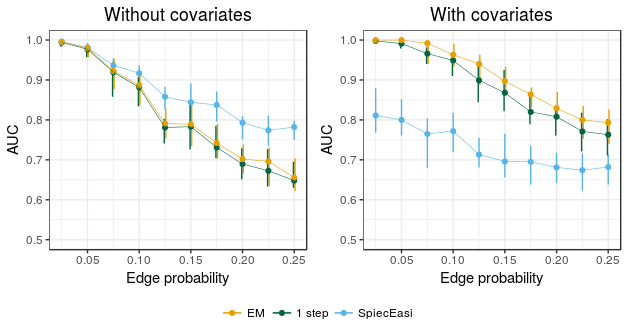
\includegraphics[width=11cm]{mosaic.png}
\end{figure}
\end{frame}
%====================================================================
%====================================================================

\section{Application}
\subsection{Oak data}

%====================================================================
%====================================================================

\begin{frame}{Oak Mildew}
\begin{columns}
\begin{column}{5cm}
\begin{figure}[htp]
\centering
\includegraphics[scale=0.07]{EA.jpg}
\caption{\textit{Pathogen Erysiphe alphitoides (EA).}}
\end{figure}
\end{column}
\begin{column}{6cm}
\begin{figure}[htp]
\centering
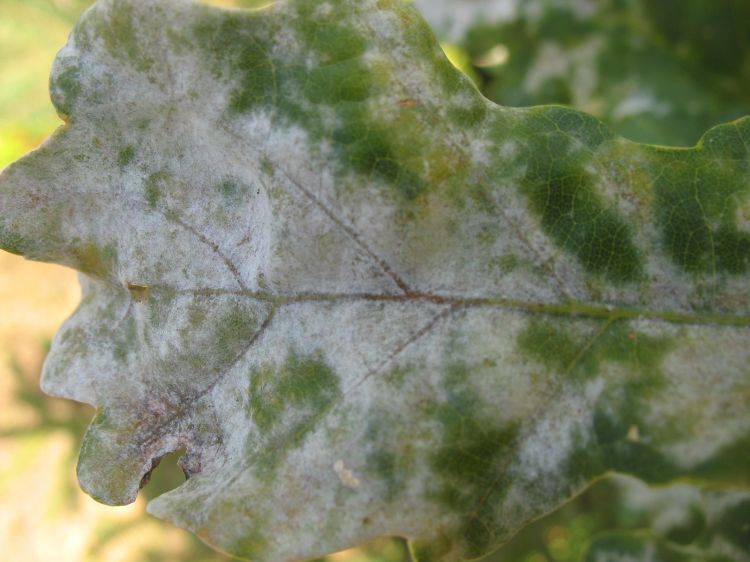
\includegraphics[scale=0.1]{mildew.jpg}
\caption{Oak leaf with powdery mildew.}
\end{figure}
\end{column}
\end{columns}
\vspace{0.5cm}
Metabarcoding of oak tree leaves microbiome \cite{jakuch}.\\

\begin{itemize}
	\item 114 sample of 94 microbial species counts (bacteria/fungi)
	\item Different read depth for bacteria and fungi: unsuited for normalization with SpiecEasi
	\item 3 quantitative covariates 
\end{itemize}
\end{frame}
%====================================================================
%====================================================================


\begin{frame}{Model with covariates}
F19: a major fungi of the microbiome.\vspace{0.3cm}
	\begin{description}
	\item[Regression coefficients]\begin{itemize}
	\item []
\end{itemize}% \begin{table}[]
%\begin{tabular}{l|lllll}
%    & Offset & \multicolumn{4}{|c}{Adding distances}   \\\cline{2-6}
%    & \multicolumn{1}{l|}{Int.}  & Int.  & to base & to trunk & to ground \\\hline
%EA  & \nega{-4.39}  &\pos{ 0.710 }&  \nega{-0.0200} &\pos{ 0.0215  } &  \nega{-0.0251  } \\
%F19 &  \nega{-4.37}  &  \nega{-8.52} & \pos{0.0219 } &  \nega{-0.0172}  & \pos{0.0143  } 
%\end{tabular}
%\end{table}

\begin{table}[]
\begin{tabular}{l|lll}
  & \multicolumn{3}{|c}{Covariates $(\times 10^{-2})$}   \\\cline{2-4}
   .  & to base & to trunk & to ground \\\hline
EA  &  \nega{-2.00} &\pos{ 2.15  } &  \nega{-2.51  } \\
F19 & \pos{2.19 } &  \nega{-1.72}  & \pos{1.43  } 
\end{tabular}
\end{table}

	\item[Degree estimation]\begin{itemize}
	\item []
\end{itemize} \begin{table}[]
\begin{tabular}{l|ll}
    & Offset & Covariates \\\hline
EA  & 2.20   & 1.86      \\
F19 & 3.03   & 2.80     
\end{tabular}
\end{table}
\end{description}
\end{frame}
%====================================================================
%====================================================================
\begin{frame}{Inferred networks}
\begin{figure}[htp]
\centering
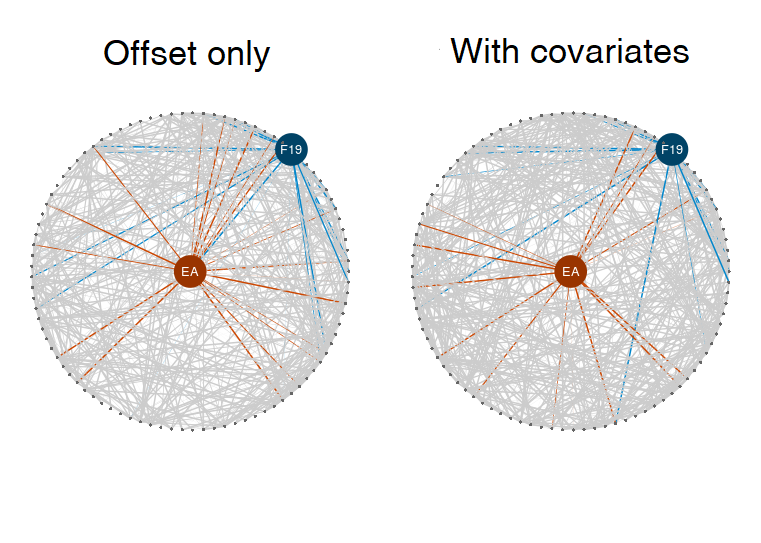
\includegraphics[width=11cm]{compare_reseaux.png}

\end{figure}

\end{frame}
%-----------------------------
%---------------------------
\section{}
\subsection{}
\begin{frame}{}
\begin{center}
\huge{\bleu{Further developments}}
\end{center}
\end{frame}

\section{Further developments}
\subsection{Other models}
\begin{frame}{Latent network models}
\large{
    \begin{itemize}
        \item 2 steps model: $\hat{\Sigma}_Z$ with {\fontfamily{qcr}\selectfont
PLNmodels}, and then network inference starting from $\hat{\Sigma}_Z$
\begin{itemize}
	\item Formal probabilistic model for network inference with \emphase{count data}
	\item  Estimation algorithm (VEM and then EM)
	\item Inclusion of \emphase{offsets} and \emphase{covariates}
    \item Yet estimating with
{\fontfamily{qcr}\selectfont
PLNmodels} adds some variability \bigskip
        \end{itemize}
        \item VEM Model: rewrite the Variational EM used in {\fontfamily{qcr}\selectfont
PLNmodels}, to incorporate the latent layer tree dependency structure.
         \begin{itemize}
             \item Would allow to re-estimate  $\hat{\Sigma}_Z$ at each iteration\bigskip
         \end{itemize}
         
         \item PLNnetworks : PLN + glasso
    \end{itemize}}
\end{frame}

\begin{frame}{Direct model}
   The {\fontfamily{qcr}\selectfont
poilog} R package computes the uni and bi-variate densities of the $\mathcal{PLN}$ distribution \vspace{0.5cm}
    \begin{itemize}
        \item \large{$\psi_{kl}(Y) = \frac{\mathds{P}(Y_k,Y_l)}{\mathds{P}(Y_k)\times \mathds{P}(Y_l)} $} \normalsize are \emphase{directly accessible}
    \end{itemize}


\begin{center}
    $\Rightarrow$ Direct network inference in the Y space\\
\end{center}
\begin{block}{Direct model}
\[\mathds{P}(Y|T) = \prod_k \mathds{P}(Y_k) \prod_{kl \in T} \mathds{P}(Y_k,Y_l)\]

\end{block}
\begin{itemize}
    \item Metropolis-Hasting simulation strategy (it works)
    \item No competitor
\end{itemize}
\end{frame}


%====================================================================
%====================================================================
\subsection{Thresholding the network}
\begin{frame}{Method for determining the threshold}
    \[Y_i  \sim Y_{\backslash -i}\]
  
   \begin{columns}
    \begin{column}{0.65\linewidth}
     \begin{itemize}
         \item Adjust each variable on all others
         \item Interpret coefficients tests in edges presence/absence: $(\mathcal{H}_0) : c_{ij} = 0$ vs  $(\mathcal{H}_1) : c_{ij} \neq 0$
         \item Deduce from the p-values an estimator of the "non-edges" number
     \end{itemize}
     \end{column}
     \begin{column}{0.35\linewidth}
      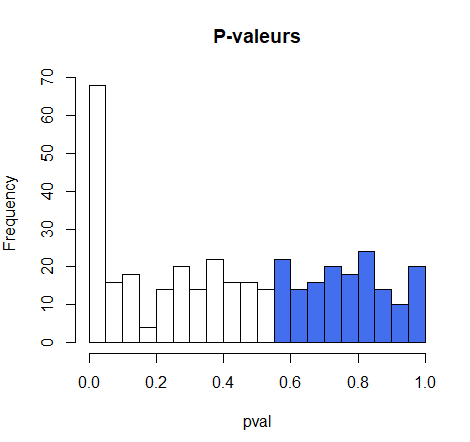
\includegraphics[width=4cm]{histpval.PNG}
     \end{column}
    \end{columns}
    \pause{
\begin{block}{$S$ and $S^*$}
 \begin{itemize}
     \item $S^*(G)$ : number of absent edges in graph $G$
     \item $S^*$ estimator: \[S(Y_G) = 2\sum \mathds{1}\{pval (Y_G) \geq 0.5 \} \]
 \end{itemize}
\end{block}}
\end{frame}
\begin{frame}{Method for determining the threshold}
\begin{figure}
    \centering
   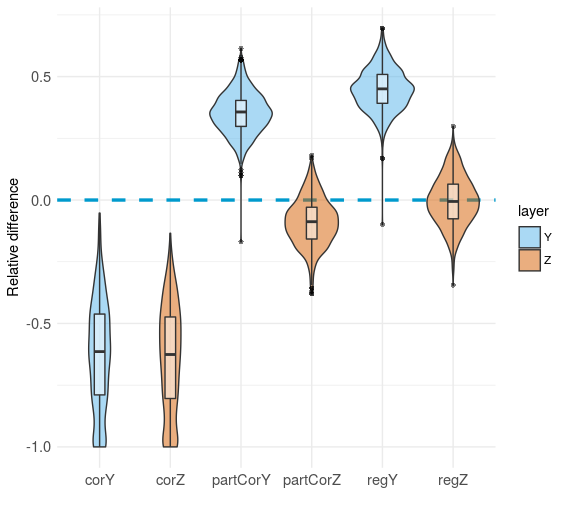
\includegraphics[width=7.5cm]{diff_estim_density.png}   
    \caption{Switching from Gaussian data Z to count data Y: relative difference between $S$ and $S^*$, related to tests of regression coefficients, correlations or partial correlations.}
\end{figure}
\end{frame}

\subsection{}

\begin{frame}{Missing major actor (species/covariable)}
Missing a major actor induces spurious edges, and distort the network interpretation \cite{LatentCWP} :
\vspace{0.2cm}
\begin{columns}
\begin{column}{0.35\linewidth}
\begin{center}
\begin{tikzpicture}
    

     %% UN graphe 
     \tikzstyle{every edge}=[-,>=stealth',shorten >=1pt,auto,thin,draw]
     \tikzstyle{every node}=[fill=yellow!40!orange]
     \tikzstyle{every          state}=[draw=none,text=white,scale=0.5,
     transform shape,circular drop shadow] 
     
     \node[fill=white] at (2.25,-0.5) ;

     % premier cluster
     \node[observed] (A1) at (1.2,0) {A};
     \node[observed] (A2) at (2.2,0) {B};
     \node[observed] (A3) at (1.7,1) {C};
     \node[observed] (A4) at (1.7,0.5) {H};
     
        \path (A2) edge [] (A4)
        (A1) edge [] (A4)
        (A3) edge [] (A4);
     

\end{tikzpicture}\\

Complete graph $\mathcal{G}$
\end{center}
\end{column}
\begin{column}{0.25\linewidth}
\begin{center}
$$\underrightarrow{marginalization}$$
\end{center}

\end{column}
\begin{column}{0.35\linewidth}
\begin{center}
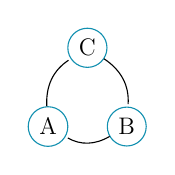
\begin{tikzpicture}
    

     %% UN graphe 
     \tikzstyle{every edge}=[-,>=stealth',shorten >=1pt,auto,thin,draw]
     \tikzstyle{every node}=[fill=yellow!40!orange]
     \tikzstyle{every state}=[draw=none,text=white,scale=0.5,
     transform shape,circular drop shadow] 
    
     
     % premier cluster
     \node[observed] (A1) at (1.2,0) {A};
     \node[observed] (A2) at (2.2,0) {B};
     \node[observed] (A3) at (1.7,1) {C};
     
        \path (A2) edge [bend left,] (A1)
        (A1) edge [bend left] (A3)
        (A3) edge [bend left] (A2);
     

\end{tikzpicture}\\


Marginal graph $\mathcal{G}_m$
\end{center}
\end{column}
\end{columns}
\vspace{0.2cm}
$$\mathbf{\mathcal{G}}\text{ }\Omega=\underbrace{\begin{pmatrix}
\Omega_{OO} & \Omega_{OH} \\ 
\Omega_{HO} & \Omega_{HH}
\end{pmatrix}}_{\text{edges from }E}  \quad \Sigma=\begin{pmatrix}
\Sigma_{OO} & \Sigma_{OH} \\ 
\Sigma_{HO} & \Sigma_{HH}
\end{pmatrix}$$
\vspace{0.4cm}
$$\mathbf{\mathcal{G}_m}\text{ : }\Omega_m= \underbrace{\Omega_{OO} - \color{red}\Omega_{OH}\Omega_{HH}^{-1}\Omega_{HO}}_{\text{edges from }E_m}\color{black} \quad \Sigma_m = \Sigma_{OO}$$

\end{frame}
%====================================================================
%====================================================================

\section{}
\subsection{}
\begin{frame}{}

\begin{center}
\huge{Thank you for your attention!}
\end{center}

\end{frame}
\appendix
\backupbegin
\begin{frame}[allowframebreaks]
\bibliographystyle{apalike}
{\footnotesize 
    \bibliography{biblio3.bib}}
\frametitle{References}
%\bibliography{cellcite}
\end{frame}\backupend
%====================================================================
%====================================================================

\end{document}